\documentclass{beamer}

\usepackage[utf8]{inputenc} % Language and font encoding
\usepackage[icelandic]{babel}
\usepackage[T1]{fontenc}


\usepackage{tikz}
\usepackage[listings,theorems]{tcolorbox}
\usepackage{booktabs}
\usepackage{minted} %Minted and configuration
\usemintedstyle{default}

\renewcommand{\theFancyVerbLine}{\sffamily \arabic{FancyVerbLine}}
%%%%%%%%%%%
% More math
%%%%%%%%%%%
\newcommand{\Mod}[1]{\ \text{mod}\ #1}

%%%%%%%%%%%%%%%%%%%%%%
% Beamer configuration
%%%%%%%%%%%%%%%%%%%%%%
\setbeamertemplate{navigation symbols}{}
\usecolortheme{dove}
\setbeamercolor{frametitle}{fg=white}

\usebackgroundtemplate%
{%
\vbox to \paperheight{

\includegraphics[width=\paperwidth]{Pics/hi-slide-head-2016}

\vfill
\hspace{0.5cm}
\includegraphics[width=0.3\paperwidth]{Pics/hi-von-logo}
\vspace{0.4cm}
    }%
}

\AtBeginSection[]
{
  \begin{frame}<beamer>
    \frametitle{Yfirlit}
    \tableofcontents[currentsection]
  \end{frame}
}

\setbeamerfont{frametitle}{size=\normalsize}
\addtobeamertemplate{frametitle}{}{\vspace*{0.5cm}}

%%%%%%%%%%%%%%%%%%%%%%%%%
% tcolorbox configuration
%%%%%%%%%%%%%%%%%%%%%%%%%

% Setup from: http://tex.stackexchange.com/a/43329/21638
\tcbset{%
    noparskip,
    colback=gray!10, %background color of the box
    colframe=gray!40, %color of frame and title background
    coltext=black, %color of body text
    coltitle=black, %color of title text 
    fonttitle=\bfseries,
    alerted/.style={coltitle=red, colframe=gray!40},
    example/.style={coltitle=black, colframe=green!20, colback=green!5},
}


%%%%%%%%%%%%%%%%%%%%%%%
% Further configuration
%%%%%%%%%%%%%%%%%%%%%%%
\hypersetup{colorlinks=true,pdfauthor={Eirikur Ernir Thorsteinsson},linkcolor=blue,urlcolor=blue}
\graphicspath{{./Pics/}}

\author{Eiríkur Ernir Þorsteinsson}
\institute{Háskóli Íslands}
\date{Haust 2016}

\title{Stærðfræðimynstur í tölvunarfræði}
\subtitle{Vika 13, fyrri fyrirlestur}

\begin{document}

\begin{frame}
\titlepage
\end{frame}


\section{Inngangur}

\begin{frame}{Í síðasta tíma}
\begin{itemize}
 \item Tré
 \item Hagnýtingar á trjám
 \item Fjöldi samanburða í röðun
 \item Trjáflakk
\end{itemize}
\end{frame}

\section{Spanntré}

\begin{frame}{Spanntré}
Oft er gagnlegt að finna spanntré (e. \emph{spanning tree}) fyrir ýmis net.
\begin{tcolorbox}[title=Spanntré]
Látum $G$ vera einfalt net. Spanntré $G$ er hlutnet $G$ sem er tré sem inniheldur alla hnúta $G$.
\end{tcolorbox}
Um spanntré gildir:
\begin{tcolorbox}
Einfalt net er samanhangandi ef og aðeins ef það hefur spanntré.
\end{tcolorbox}
Tré hefur eitt spanntré (tréð sjálft). Önnur einföld samanhangandi net hafa fleiri spanntré.
\end{frame}

\begin{frame}{Af hverju spanntré?}
\begin{itemize}
 \item Spanntréð sjálft getur haft merkingu
 \begin{itemize}
  \item Dæmi: Snjóstormur hefur lamað vegakerfið, spanntré lýsir þeim vegum sem nægilegt er að ryðja til að umferð komist aftur í gang
 \end{itemize}
 \item Tré eru oft meðfærilegri heldur en almenn net
 \begin{itemize}
  \item Getum viljað búa til tré úr neti til að geta notað öflug trjáreiknirit á það
 \end{itemize}
\end{itemize}
\end{frame}


\begin{frame}{Að finna spanntré}
\begin{itemize}
 \item Einföld leið til að finna spanntré í netinu: 
 \begin{itemize}
  \item Finna allar einfaldar rásir í netinu
  \item Fjarlægja leggi úr rásunum þar til einungis tré verður eftir
 \end{itemize}
 \item Þessi leið er hins vegar ekki skilvirk, því við þurfum fyrst að finna allar einföldu rásirnar
 \item Skoðum tvær leiðir:
 \begin{itemize}
  \item Dýptarleit (e. \emph{depth-first search})
  \item Breiddarleit (e. \emph{breadth-first search})
 \end{itemize}
\end{itemize}
\end{frame}

\begin{frame}{Dýptarleit}
\begin{itemize}
 \item Getum lauslega lýst dýptarleit að spanntré í einföldu samanhangandi neti á eftirfarandi hátt:
 \begin{itemize}
  \item Veljum hnút í netinu til að vera rót
  \item Myndum veg í netinu með því að bæta endurtekið við nýjum hnút sem er aðlægur síðasta hnút sem við bættum við (ásamt leggnum sem tengir hnútana tvo saman)
  \begin{itemize}
   \item Þessi vegur er byrjunin á spanntrénu
  \end{itemize}
  \item Ef vegurinn inniheldur ekki alla hnúta netsins bökkum við eftir veginum þar til við finnum aðlægan hnút sem við höfum ekki heimsótt og myndum nýjan veg sem hefst þar
 \end{itemize}
 \item Athugum að þessi leit er endurkvæm!
\end{itemize}
\end{frame}

\begin{frame}{Dæmi}
\begin{center}
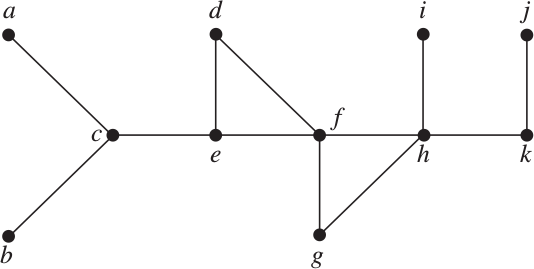
\includegraphics[width=0.7\textwidth]{tree-spanning-dfs}

\pause
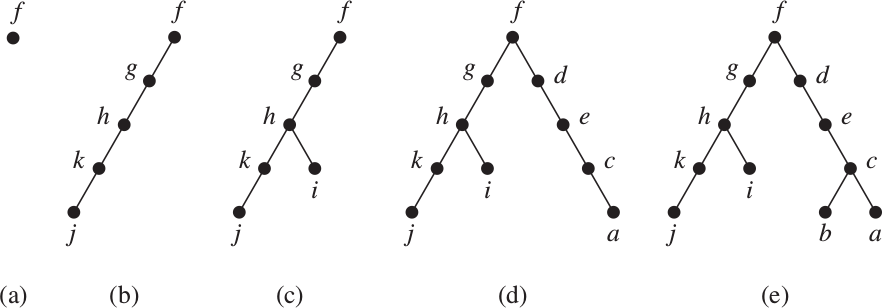
\includegraphics[width=0.9\textwidth]{tree-spanning-dfs-procedure}
\end{center}

\end{frame}

\begin{frame}{Breiddarleit}
\begin{itemize}
 \item Getum lauslega lýst breiddarleit að spanntré í einföldu samanhangandi neti á eftirfarandi hátt:
 \begin{itemize}
  \item Veljum hnút í netinu til að vera rót spanntrés
  \item Bætum öllum nágrönnum (ásamt tilheyrandi leggjum) við spanntréð og skilgreinum fyrir þá röðun, munum fjarlægð þeirra frá rótinni
  \item Skoðum endurtekið og í skilgreindri röð alla nágranna þeirra hnúta sem voru í síðustu fjarlægð frá rótinni og bætum þeim við spanntréð ef við höfum ekki gert það áður
 \end{itemize}
 \item Líka endurkvæmt!
\end{itemize}
\end{frame}

\begin{frame}{Dæmi}
\begin{center}
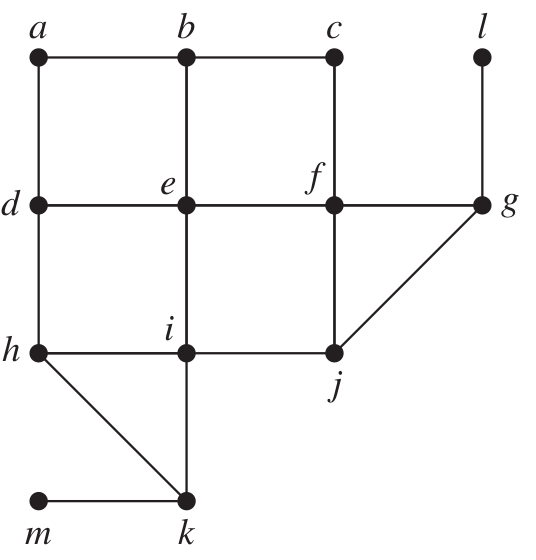
\includegraphics[width=0.4\textwidth]{tree-spanning-bfs}

\pause
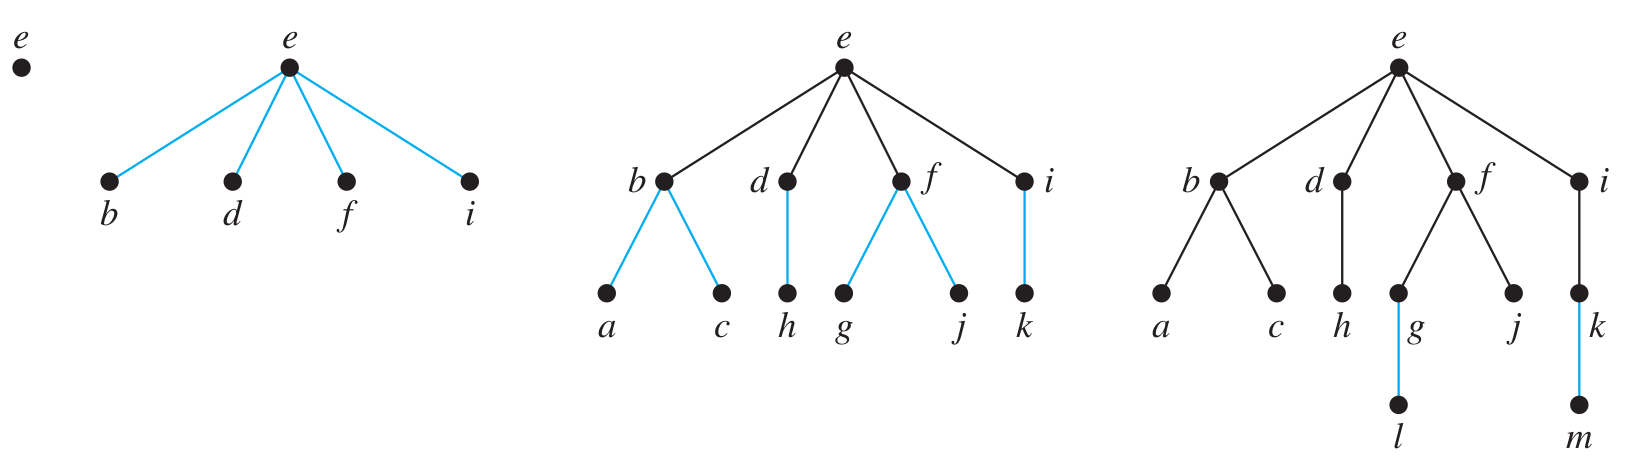
\includegraphics[width=0.9\textwidth]{tree-spanning-bfs-procedure}
\end{center}

\end{frame}

\begin{frame}{Spanntré í stefndum netum}
\begin{itemize}
 \item Við getum notað breiddarleit eða dýptarleit til að mynda ``spannskóg'' í stefndu neti
 \item Byrjum á nýjum samhengisþætti þegar enginn örvaleggur finnst
\end{itemize}
\end{frame}

\section{Léttustu spanntré}

\begin{frame}{Léttustu spanntré}
\begin{tcolorbox}[title=Léttustu spanntré]
Léttasta spanntré í samanhangandi vegnu neti er spanntré netsins sem hefur lægstu mögulegu summu leggjaþyngda.
\end{tcolorbox}
Setjum fram tvö gráðug reiknirit til að finna léttustu spanntré.
\end{frame}

\begin{frame}{Reiknirit Prims}
\begin{itemize}
 \item Reikniritið er venjulega kennt við Robert Prim (1957), en var fyrst fundið upp af Vojtěch Jarník (1930)
 \item Reikniritið er gráðugt, finnur léttasta spanntré (í neti með $e$ hnútum og $v$ leggjum) og er eftirfarandi:
 \begin{itemize}
  \item Finnum legg af lágmarksþyngd í netinu, setjum hann í leggjamengi spanntrésins
  \item Bætum endurtekið við legg af lágmarksþyngd sem er aðlægur hnúti sem bæði snertir legg í spanntrénu og myndar ekki rás í spanntrénu
  \item Hættum þegar $v-1$ leggjum hefur verið bætt við, bætum þá við öllum hnútunum
 \end{itemize}
 \item Reikniritið keyrir á $O(e \log v)$ tíma
\end{itemize}
\end{frame}

\begin{frame}{Reiknirit Kruskals}
\begin{itemize}
 \item Kennt við Joseph Kruskal, er líka gráðugt reiknirit sem finnur léttasta spanntré (í neti með $e$ hnútum og $v$ leggjum)
 \begin{itemize}
  \item Finnum legg af lágmarksþyngd í netinu, setjum hann í leggjamengi spanntrésins
  \item Bætum endurtekið við legg af lágmarksþyngd sem myndar ekki rás í spanntrénu
  \item Hættum þegar $v-1$ leggjum hefur verið bætt við, bætum þá við öllum hnútunum
 \end{itemize}
 \item Reikniritið keyrir á $O(e \log e)$ tíma
\end{itemize}
\end{frame}

\begin{frame}{Næst}
\end{frame}


\end{document}
